\documentclass[a4paper, UTF8]{ctexart}
\usepackage{ctex}
\usepackage{amsmath}
\usepackage{amsthm}
\usepackage{multirow}
\usepackage{amssymb}
\usepackage{graphicx}
\usepackage{geometry}
\usepackage{bm}
\usepackage{subfigure}
\usepackage{float}
\usepackage{mathrsfs}
\renewcommand\thesection{\arabic{section}}
\newtheorem*{exercise}{\textbf{习题}}
\newtheorem*{theorem}{Theorem}
\title{Manifole Learning Homework 6}
\date{\today}
\author{安捷 1601210097}
\begin{document}
\maketitle
  \begin{exercise}[95]
    \begin{proof}
      由于 $k_1$ 是一个核函数,因此由Mercer定理,对于任意的 $L_2$可积函数 $g$有
      \begin{equation}
        \int g \left( \mathbf{x} \right) g \left(  \mathbf{y}\right)k_1 \left( \mathbf{x}, \mathbf{y} \right) d \mathbf{x} d \mathbf{y} > 0
      \end{equation}
      而由于 $k \left( \mathbf{x}, \mathbf{y} \right) = \mathrm{exp}\left( k_1 \left( \mathbf{x}, \mathbf{y} \right) \right) > k_1 \left( \mathbf{x}, \mathbf{y} \right)$,因此有
      \begin{equation}
        \int g \left( \mathbf{x} \right) g \left( \mathbf{y} \right) k \left( \mathbf{x}, \mathbf{y} \right) d \mathbf{x} d \mathbf{y} > \int g \left( \mathbf{x} \right) g \left( \mathbf{y} \right) k_1 \left( \mathbf{x}, \mathbf{y} \right) d \mathbf{x} d \mathbf{y} > 0
      \end{equation}
      由Mercer定理, $k \left( \mathbf{x}, \mathbf{y} \right)$ 是核函数。
    \end{proof}
  \end{exercise}
  \begin{exercise}[96]
    计算得到的准确率为
    \begin{table}[htbp!]
      \centering
      \begin{tabular}{l}
        degree of polynomial= 1 accuracy= 1.0 \\
        degree of polynomial= 2 accuracy= 0.8947368421052632 \\
        degree of polynomial= 3 accuracy= 0.8947368421052632 \\
        degree of polynomial= 4 accuracy= 0.8947368421052632 \\
        degree of polynomial= 5 accuracy= 0.8947368421052632 \\
      \end{tabular}
      \caption{$\epsilon_1=100, \epsilon_2 = 32000$时预测准确率}
    \end{table}
  \end{exercise}
  \begin{exercise}[98]
    \begin{figure}[htbp!]
      \centering
      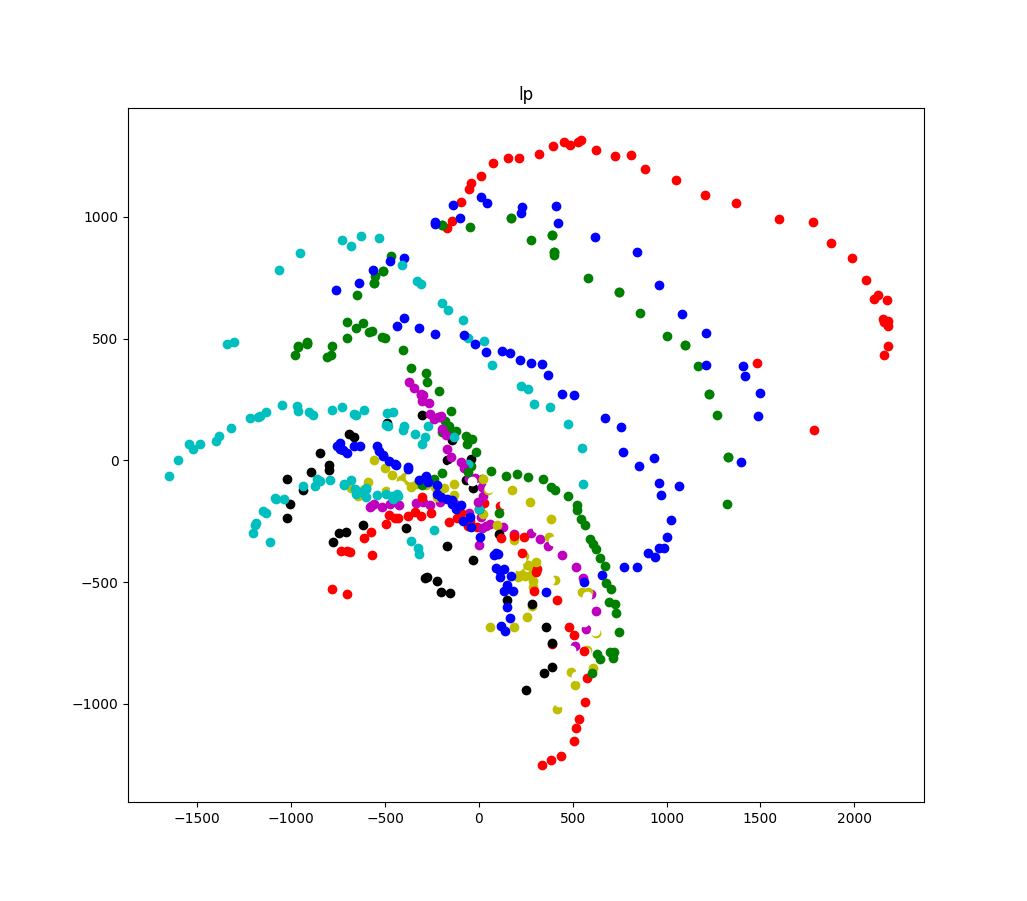
\includegraphics[width=0.8\textwidth]{fig77_1.png}
      \caption{CMDS结果图}
    \end{figure}
    \begin{figure}[htbp!]
      \centering
      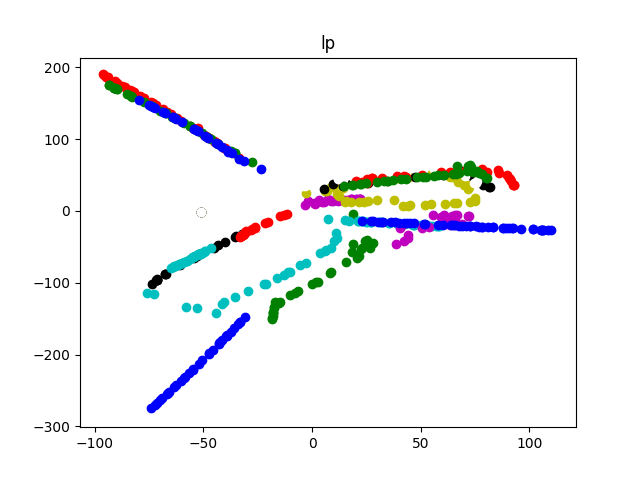
\includegraphics[width=0.8\textwidth]{fig98.png}
      \caption{isomap结果图}
    \end{figure}
    从图中明显可以看出,isomap使得同一个人的照片基本处于一条直线上,因此,效果要明显好于CMDS算法。
  \end{exercise}
  \clearpage
  \begin{exercise}[100]
    由Language乘子法及KKT条件可得,(5.28)的解为满足下式的 $\mathbf{a}$
    \begin{equation}
      \frac{\mathbf{X}^T \left( \mathbf{X}\mathbf{a} - \mathbf{x}_i \right)}{\lVert \mathbf{X} \mathbf{a} - \mathbf{x}_i \rVert} = \lambda
    \end{equation}
  其中,上式中的参数 $\lambda$ 可以通过
  \begin{equation}
    \sum_j \mathbf{a}_j = 1
  \end{equation}
  求得,实际上,此时有
  \begin{equation}
    \mathbf{a}_i = 1, \mathbf{a}_j = 0
  \end{equation}
  显然这与weight matrix construction得到的结果不相同,对后者的数值计算结果参见相关代码。 $\mathbf{W_0}$的计算结果如下
  \begin{table}[htbp!]
    \centering
    \begin{tabular}{c}
      1.01220703 \\
       0.01696777 \\
       0.01464844 \\
       0.04541016 \\
       0.04833984 \\
       0.00756836 \\
       0.02404785 \\
       0.02282715 \\
       0.02600098 \\
       0.01843262 \\
       0.0123291  \\
       0.01574707 \\
       0.03015137 \\
       0.01586914 \\
       0.02868652 \\
       0.01367188 \\
       0.01782227 \\
       0.02600098 \\
       0.0123291  \\
       0.03881836 \\
       0.02502441 \\
       0.02099609 \\
       0.02587891 \\
       0.02587891 \\
       0.02636719 \\
       0.01477051 \\
       0.01452637 \\
       0.02734375 \\
       0.02514648 \\
       0.02966309 \\
       0.02990723 \\
       0.01757812 \\
      -0.0098877  \\
       0.00708008 \\
       0.0246582  \\
       0.02478027 \\
       0.01147461 \\
       0.01208496 \\
    \end{tabular}
    \caption{$\mathbf{W_0}$}
  \end{table}
  显然与第一种计算方法得到的结果不同但是较为接近。
  \end{exercise}
\end{document}
